\documentclass{VUMIFInfKursinis}
\usepackage{algorithmicx}
\usepackage{algorithm}
\usepackage{algpseudocode}
\usepackage{amsfonts}
\usepackage{amsmath}
\usepackage{bm}
\usepackage{color}
\usepackage{hyperref}  % Nuorodų aktyvavimas
\usepackage{url}

\usepackage{subcaption} % For subfigures
\usepackage{enumitem} % For 1.1 numbering in lists
\setlist[enumerate]{label*=\arabic*.}
\usepackage{multicol}
\usepackage{graphicx}


\usepackage[font=small,labelfont=bf]{caption} 
\captionsetup[figure]{position=bottom}


% Titulinio aprašas
\university{Vilniaus universitetas}
\faculty{Matematikos ir informatikos fakultetas}
\department{Informatikos katedra}
\papertype{Kursinis darbas}
\title{Dokomentų klasterizacija}
\titleineng{Document clustering}
\status{4 kurso 1 grupės studentas}
\author{Dominykas Ablingis}
\supervisor{Prof., Dr. Rimantas Kybartas}
\date{Vilnius \\ \the\year}


% Nustatymai
\bibliography{bibliografija} 


%My macros                                                                                                                                                                                                                                                                                                                                                                              
\newcommand{\ltang}[2]{#1 (angl. \textit{#2})}                                                                                                                                             
\newcommand{\BigO}[1]{$\mathcal{O}(#1)$}


\begin{document}
\maketitle

\tableofcontents

\sectionnonum{Įvadas}
Šiais laikais sparčiai vystantis informacinėms technologijoms ir
gausėjant informacijos kiekiams, vis aktualesnė tampa kokybiška ir
greita reikiamos informacijos paieška, jos organizavimas ir naujų
įžvalgų išgavimas. Darbą su dideliais tekstinės informacijos kiekiais
galėtų pagreitinti ir palengvinti įprastai skaitmeninių duomenų analizei
naudojami klasterizavimo metodai.

Šio darbo tikslas yra išnagrinėti ir aprašyti klasterizavimo metodus,
tekstinių duomenų parengimą darbui su klasterizavimo algoritmais bei
gautų klasterių kokybės įvertinimo kriterijus.




\subsection*{Duomenų analizės eiga}

Klasterizavimas tėra vienas iš žingsnių tekstinių duomenų analizės
procese. Tekstinių duomenų analizės procesą galime suskirstyti į keletą
žingsnių \cite{fayyad1996data}:


\begin{enumerate}
\item
  \ltang{Probleminės srities nustatymas}{problem domain}. 
\item
  \ltang{Duomenų surinkimas}{data collection}.
\item
  \ltang{Duomenų tvarkymas ir apdorojimas}{cleaning and
  preprocessing}\footnote{3 ir 4-tas žingsniai gali būti apibrėžti kaip
     \ltang{požymių pasirinkimas}{feature selection}. Svarbu
    atrinkti požymius, kurie yra esminiai atskiriant objektus ir juose
    būtų konkreti informacija užduočiai atlikti, tuo pačiu stengiantis
    palikti kuo mažiau perteklinės informacijos ir neprarasti svarbios
    informacijos.}.
\item
  \ltang{Duomenų supaprastinimas ir transformavimas}{reduction and
  projection}.
\item
  \ltang{Duomenų analizavimas}{data analysis}. Klasterizavimo
  atveju tai būtų tinkamo klasterizavimo algoritmo parinkimas ir
  taikymas. Kadangi egzistuoja didelė klasterizavimo algoritmų įvairovė,
  jie skiriasi ne tik veikimo principu, bet ir gautų rezultatų forma,
  todėl norint išsirinkti tinkamą algoritmą, reikia įvertinti tiek
  turimus duomenis, tiek norimus gauti rezultatus.

  \begin{enumerate}
  \item
    \ltang{Panašumo matas}{proximity measure} – tai kiekybinis
    matas, kuris įvertina kiek du požymių vektoriai yra „panašūs“ ar
    „nepanašūs“ tarpusavyje. Reikėtų pasitikrinti, ar visi požymiai yra
    lygiaverčiai ir tarp jų nėra dominuojančių.
  \item
	\ltang{Panašumo matas}{proximity measure}
	 – turėtų nurodyti, kokius klasterius tikimasi išskirti
    duomenų aibėje, taip pat duomenų jungimo į vieną klasterį ir
    atskyrimo į kelis klasterius kriterijus.
  \end{enumerate}
\item
  \ltang{Rezultatų validavimas / įvertinimas }{ validation of
  results} – klasterizavimo proceso rezultatų formalus teisingumo
  įvertinimas. Tam yra naudojami specifiniai metodai.
\item
  \ltang{Rezultatų interpretavimas}{ interpretacion of results} –
  nors gauti galutiniai klasteriai gali atitikti matematinius
  reikalavimus, bet gauti rezultatai gali prieštarauti sveikam protui.
  Visgi rezultatas tėra galimas duomenų suskirstymas į grupes, todėl
  dažniausiai gautus rezultatus reikia lyginti su iš anksto sudaryta
  hipoteze.
\item
  Rezultatų panaudojimas. Tai gali būti vienas iš didesnės analizės
  žingsnių arba konkretus rezultatas padedantis priimti sprendimą.
\end{enumerate}

Šiame ir projektiniame darbe apžvelgsiu 2 – 6-tą žingsnius, daugiausia
dėmesio skirdamas 5-tam žingsniui.











\section{Tekstinių dokumentų parengimas klasterizavimui}

Ši proceso dalis atsakinga už tai, kad tekstai iš žmogui patogios formos
būtų paversti į formą patogią duomenų analizei, šiuo atveju,
klasterizavimui. Šis procesas atliekamas tokiais žingsniais:

\begin{itemize}
\item
  \textbf{Informacijos išgavimas} – šiame žingsnyje įvairių formų
  (pvz., nuotraukos, audio įrašai) ir formatų (pvz., HTML, PDF, EPUB)
  dokumentus paverčiame į patogius analizei tekstus. Pašaliname
  formatavimą, paveiksliukus, išdėstymą ir kitą informaciją, kurią sunku
  paversti į vertingą tekstą.
\item
  \textbf{Teksto filtravimas} – šiame žingsnyje panaikiname analizei
  nereikalingą tekstinę informaciją, supaprastiname ir suvienodiname
  žodžius \cite{mugunthadevi2011survey}.

  \begin{itemize}
  \item
    \textbf{Leksikos analizė} – suskaidome tekstą į atskirus žodžius ir
    pašaliname simbolius, skyrybos ženklus ir skaičius.
  \item
    \textbf{Nereikšmingų žodžių pašalinimas} – pašaliname žodžius,
    kurie nėra vertingi analizei. Tai gali būti mažai reikšmės turintys
    žodžiai, kurie labiau reikalingi „suklijuoti“ tekstą patogesniam
    skaitymui. Taip pat pašalinami praktiškai kiekviename dokumente
    sutinkami žodžiai, kurie nesvarbūs klasterizavimui.
  \item
    \textbf{Sinonimiškumas ir daugiareikšmiškumas} – bandome rasti
    sinonimiškiems žodžiams vieną bendrą žodį ar daugiareikšmius žodžius
    paversti į konkretesnius.
  \item
    \textbf{Morfologinis analizavimas} – skirtingas žodžio formas
    suvienodiname į vieną bendrinę formą. Tai atliekama išgaunant žodžio
    šaknį arba bandant paversti jį į bendrinę formą, dar žinomą kaip
    lema.
  \end{itemize}
\item
  \textbf{Požymių išskyrimas} – turimus filtruotus tekstinius duomenis
  reikia paversti į skaitinius, nes su tokiais dirba dauguma
  klasterizavimo algoritmų \cite{alelyani2013feature}. Tai atliekame dokumentus paversdami į
  vektorius, kuriuose kiekvienas elementas atitinka visame dokumentų
  rinkinyje sutinkamus žodžius. Elementų reikšmės nurodo arba žodžio
  buvimą (binarinė reikšmė) tekste, arba kaip dažnai jie sutinkami
  (skaliarinė reikšmė).
\end{itemize}











\section{Klasterizavimas}

Klasteris – tai panašių objektų grupė \cite{tan2007introduction}.
Klasterinė analizė tai yra matematinių metodų visuma, kurios pagalba
galima objektų arba reikšmių aibes pagal jų panašumus, suskirstyti į
prasmingas grupes – klasterius. Tai atliekama be jokios papildomos
informacijos apie tas grupes (jų dydį, kiekį, grupavimo požymius).
Taigi, klasterių analizė yra iš anksto nežinomų struktūrų paieška. Iš to
kyla pagrindinis klasterizavimo iššūkis ir privalumas – sugebėjimas
atrasti sudėtingas struktūras be išankstinės informacijos apie jas.
Kitaip tariant, pagrindinis klasterizavimo tikslas – maksimizuoti
objektų, esančių toje pačioje grupėje, tarpusavio panašumą ir
minimizuoti objektų, esančių skirtingose grupėse, panašumą.

Dokumentų klasterizavimas yra labai dažnai painiojamas su dokumentų
klasifikavimu (dar vadinamas kategorizavimu). Klasifikuojant duomenis iš
anksto apibrėžiamos kategorijos ir priklausomai nuo duomenų turinio, jie
yra priskiriami kuriai nors iš tų kategorijų (dažnai vadinamų klasėmis),
todėl duomenų klasifikacija yra priskiriama \ltang{prižiūrimo mokymosi}{supervised learning} užduotims. 
Tuo tarpu klasterizuojant
duomenis, jokios iš anksto apibrėžtų kategorijų aibės nėra, todėl
klasterizavimas yra priskiriamas \ltang{neprižiūrimo mokymosi}{unservised learning} užduotims.






\subsection{Panašumo funkcijos / įverčiai}

Nors turime klasterio apibrėžimą, bet vis dar neaišku kaip jį panaudoti
tekstiniams duomenims, kaip apibrėžti dviejų dokumentų panašumą (ar
skirtingumą). Ankstesniame skyriuje apibūdinome kaip tekstinį dokumentą
paversti į skaitinius duomenis, sekantis žingsnis būtų dokumentų
panašumo nustatymas, pasinaudojus panašumo ir metrikinėmis
funkcijomis\footnote{Metrika yra matematinis terminas, apibūdinantis
  atstumą matuojančias funkcijas. Todėl ne bet kurią funkcija galima
  vadinti metrika, ji turi atitikti reikalavimus \cite{daeoms}.}
Aptarsime dalį populiariausių klasterizavimo srityje naudojimų metrikų
ir panašumo matavimo matų \cite{huang2008similarity}.

\textbf{Euklido atstumas} tarp taško x ir taško y – tai trumpiausias atstumas
tarp šių taškų. Plokštumoje arba trimatėje erdvėje – tai taškus
jungianti tiesė. Bendru n-matės erdvės atveju šis atstumas
apskaičiuojamas pagal formulę:

$$ \mathrm{d_{Euklido}} (q,p) 
	= {\sqrt {(q_{1}-p_{1})^{2}+(q_{2}-p_{2})^{2}+\cdots +(q_{n}-p_{n})^{2}}}
	=\sqrt {\sum _{i=1}^{n}(q_{i}-p_{i})^{2}} $$

Tai pati populiariausia metrika \cite{jain1988algorithms}, bet ji turi problemų, kai
matmenys turi skirtingą svarbą, taip pat kai du dokumentai yra su
identišku turiniu, bet skirtingais ilgiais, bus laikomi skirtingais.

\textbf{Manheteno atstumas} (dar žinomas kaip miesto kvartalų atstumas)
– absoliučių skirtumų tarp visų porų reikšmių suma ir skaičiuojamas
pagal formulę:

$$ \mathrm{d_{Manhateno}} (q,p)
	=\sum _{i=1}^{n}|q_{i}-p_{i}|^2 $$

\textbf{Čebyševo atstumas} – didžiausias absoliutus skirtumas tarp visų
porų. Jis skaičiuojamas taip:

$$ \mathrm{d_{Čebyševo}} (q,p)
	=\max_i|q_{i}-p_{i}| $$

\begin{figure}[H]
  \centering
  \begin{subfigure}[b]{0.4\textwidth}
  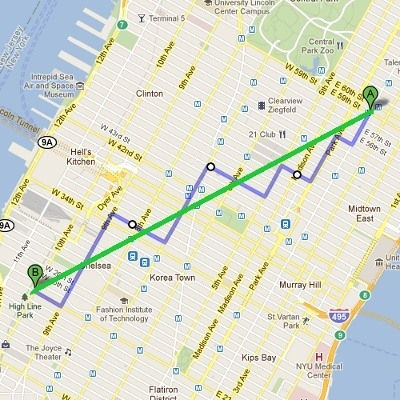
\includegraphics[width=\textwidth]{img/MvsE}
  \caption{}
  \end{subfigure}
  %
  \begin{subfigure}[b]{0.4\textwidth}
  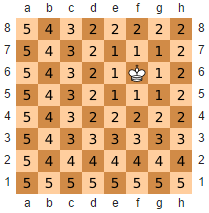
\includegraphics[width=\textwidth]{img/cheb}
  \caption{}
  \end{subfigure}
  \caption{a – Manhateno (mėlina linija) ir eukliko (žalia linija) atstumų palyginimas reliame pasaulyje.\\
           Šaltinis: \url{https://arc.cs.rutgers.edu/courses/f17/lecture.08.extra.pdf}\\
           b – Čebyševo atstumas atitinka karaliaus galimus ėjimus šakmatų žaidime.\\
           Šaltinis: \url{http://www.ieee.ma/uaesb/pdf/distances-in-classification.pdf}}
\end{figure}

\textbf{Minkovskio atstumas} – apibendrina skirtingų atstumų metrikas. Parinkus
skirtingas p reikšmes, galima gauti šiuos atstumus: p = 1 Manheteno, p =
2 Euklido, p $\to$ ∞ Čebyševo:

$$ \mathrm{d_{Minkowski}} (q,p)
	= \left(\sum _{i=1}^{n}|q_{i}-p_{i}|^2 \right)^{1/p} $$

\textbf{Kosinuso koeficientas} – kampas tarp dvejų vektorių.
Mūsų atveju, vektoriai negali būti neigiami, tai šios funkcijos reikšmių
sritis yra $[0, 1]$. $0$ reiškia, kad abu dokumentai neturi
bendrų terminų, $1$ – abu dokumentai turi identiškus terminus (bet
nebūtinai identiškus kiekius).

Jei dirbame su žodynais be svorių, galime naudoti aibėms skirtą versiją:

$$ \mathrm{d_{Cosinuso}} (q,p)
	=\frac{|Q \cap P|}{\sqrt{|Q|×|P|}} $$

Jei dirbame su svoriais:

$$ \mathrm{s_{Cosinuso}} (q,p)
	={\mathbf {Q} \cdot \mathbf {P}  \over \|\mathbf {Q} \|\|\mathbf {P} \|}
	={\frac {\sum \limits _{i=1}^{n}{Q_{i}P_{i}}}{{\sqrt {\sum \limits _{i=1}^{n}{Q_{i}^{2}}}}{\sqrt {\sum \limits _{i=1}^{n}{P_{i}^{2}}}}}}$$

Kosinuso koeficientas yra vienas populiariausių panašumo matų \cite{larsen1999fast}.
Pagrindinis jo privalumas, kad jis identiškais laiko skirtingo dydžio
dokumentus su vienodomis struktūromis, todėl išvengia didelio matmenų
kiekio problemos.

\begin{figure}[H]
  \centering
  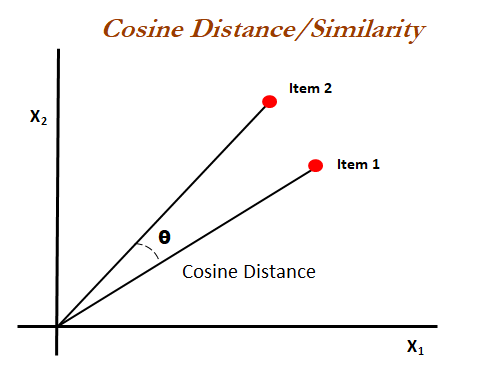
\includegraphics[scale=.5]{img/cos}
  \caption{Kosinuso panašumas tarp dvejų taškų.\\
           Šaltinis: \url{https://www.safaribooksonline.com/library/view/statistics-for-machine/9781788295758/eb9cd609-e44a-40a2-9c3a-f16fc4f5289a.xhtml}}
\end{figure}






\subsection{Klasterizavimo algoritmai}

Egzistuoja plati klasterizavimo algoritmų įvairovė (pvz.: \ref{clustAlg} pav.), todėl atsiranda
poreikis kaip nors juos suskirstyti. Vienas iš būdų – pagal sudarytų
klasterių savybes:

\begin{itemize}
\item
  \ltang{\textbf{Griežti}}{exclusive, hard} – kai klasteriai
  neturi bendrų narių. Kartais gali atsirasti atvejai, kai elementas
  „matematiškai“ gali priklausyti ne vienai grupei, bet toks atvejis
  yra retas.\\
  \ltang{\textbf{Negriežti}}{non-exclusive, soft, fuzzy} – kai
  klasteriai tarpusavyje gali turėti bendrų narių. Tokiu atveju galime
  nagrinėti, kaip konkretus elementas priklauso skirtingoms grupėms ir
  kaip gerai jas atitinka.
\item
  \ltang{\textbf{Plokšti}}{flat} – kai elementai suskirstomi į
  grupes, kurios viena kitai yra lygios.\\
  \ltang{\textbf{Hierarchiški}}{hierarchical, taxonomic} – kai
  grupė gali būti sudaryta iš kelių „konkretesnių“ grupių. Pvz.,
  retryveris $\to$ šuo $\to$ žinduolis $\to$ gyvūnas.
\end{itemize}

Kitas būdas – skirstyti algoritmus į grupes pagal veikimo principą \cite{kadhim2014text}.
Toliau šiame darbe bus aprašomi populiariausi keturių tipų algoritmai.






\subsubsection{K-vidurkiai}\label{km}

\ltang{K-vidurkių}{k-means} algoritmas priklauso \ltang{skirstant}{partitional clustering}
arba centroidais\footnote{Taškai
apibūdinantys klasterį, bet nebūtinai jam priklausantys.} paremtu
klasterizavimu grupėmis \cite{macqueen1967some}. Dažniausiai šis algoritmas pradeda nuo
atsitiktinių klasterių ir juos gerina vis keisdamas centroidų padėtį.

Veikimo principas:

\begin{enumerate}
\item
  Sukuriami $k$ centroidai. („Inicijavimo metodai“ poskyryje
  detaliau apie tai).
\item
  Objektai priskiriami artimiausiam (pagal matavimo matą) centroidui.
  Taip sudaromi klasteriai.\label{km2step}
\item
  Išsaugome sumą atstumų tarp centroidų ir jiems priklausančių objektų
  (toliau $Cdis$).
\item
  Apskaičiuojame klasterio naują centrą pagal jam priskirtus objektus.
  Jeigu centroido pozicija pasikeitė, einam į \ref{km2step}-ą žingsnį, jeigu ne –
  sustojam.
\end{enumerate}

\begin{figure}[H]
  \centering
  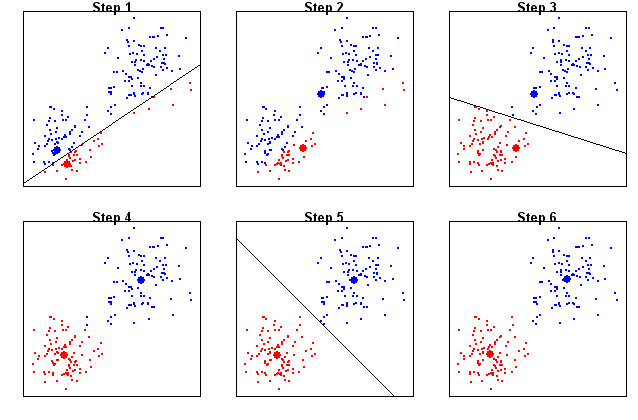
\includegraphics[scale=.5]{img/Kmean}
  \caption{1,3,5 žingsniai parodo dalijimo procesą; 2,4,6 – perskaičiavimo\\
           Šaltinis: \url{https://medium.com/@dilekamadushan/introduction-to-k-means-clustering-7c0ebc997e00}}
\end{figure}

K-vidurkių metodas dažniausiai randa lokalų maksimumą, o globalaus
maximumo suradimas yra NP – sudėtinga problema. Ji dažniausiai
sprendžiama kelis kartus kartojant algoritmą su skirtingomis inicijavimo
reikšmėmis ir parenkant tą, kuri grąžina mažiausią $Cdis$.

Dėl palygint greito konvergavimo ir paprasto veikimo, šis algoritmas
tapo vienas populiariausių klasterizavimo algoritmų
\cite{wu2008top}.
Tačiau ne vieną kartą pastebėta, jog taikant K-vidurkių metodą,
algoritmo iteracijų skaičius yra kur kas mažesnis nei klasterizuojamų
objektų skaičius. Norint gauti kokybiškus klasterius, svarbios geros
$k$ reikšmės ir pradinės centroidų padėties parinkimas.

\subsubsubsection*{K parinkimas}

Nors kai kurioms problemoms spręsti mes iš anksto galime žinoti
$k$, bet daugumai problemų šis sprendimas gali atrodyti
atsitiktinis. Vis didinat $k$ reikšmę $Cdis$ sumažėtų ir mūsų
modelis būtų vis „tikslesnis“, kol galiausiai kiekvienas objektas
turėtų atskirą klasterį.

Vienas iš sprendimų yra \ltang{„bausti“}{penalize} sudėtingumą.
$Sum$ = $Cdis$ + $Complexity$. Nes didinat $k$,
$Cdis$ mažėja vis lėčiau, galiausiai didėjantis $Complexity$
pradeda didinti $Suma$ reikšmę ir tada sustojame didinti $k$.
Yra keletas skirtingų $Complexity$ apskaičiavimo funkcijų. Viena
žinomiausių yra X-Means \cite{pelleg2000x}.

\subsubsubsection*{Centroidų inicijavimo metodai:}

\begin{enumerate}
\item
  Atsitiktinis – dažniausiai parenkama atsitiktinio objekto padėtis.
  Tai garantuoja, kad centroidai bus šalia duomenų, bet tuo pačiu
  padidėja šansas, kad bus parinkti šalimais esantys elementai.
\item
  \ltang{Atstumu paremti}{distance-based} – pirmą centroidą
  parenkame atsitiktinai, tada surandame tolimiausią tašką nuo jo ir jį
  parenkame kitu centroidu, tada parenkame tolimiausią nuo dviejų esamų
  centroidų ir taip toliau. Nors tai išsprendžia problemą su šalimais
  esančiais klasteriais, bet šiuo atveju didelė tikimybė, kad bus
  parinkti \ltang{atsiskyrėliai taškai}{outlier}. 
\item
  k-means++ (atsitiktinis + atstumo) \cite{arthur2007k} – parenka pirmą
  centroidą atsitiktinai, tada antrą vėl parenka atsitiktinai, bet šį
  kartą papildomai pritaikę svorį, proporcingą atstumui iki artimiausio
  centroido, pakeltą kvadratu ir kartojame iš naujo. Šis metodas parenka
  centroidus, kurie yra tolimai nuo kitų, bet kartu yra tankiose
  vietose.
\end{enumerate}

\subsubsubsection*{K-vidurkio algoritmo savybės:}

\begin{itemize}

\item
  Sudėtingumas.
\item
  Sugeneruoja griežtus, plokščius klasterius. 
\item
  Sudaryti klasteriai yra sferinės formos, atitinka voronoi diagramas \ref{img:voronoi}.
\item
  Privalome iš anksto nurodyti $k$ pradinę reikšmę ir centroidų
  pradinę padėtį\footnote{Tai iš dalies prieštarauja klasterizavimo
    principui, kad klasterizavimas turi būti atliktas be papildomos
    informacijos.}.
\item
  Dėl palyginti spartaus veikimo ir paprastos realizacijos šis
  algoritmas rekomenduojamas kaip pirmas klasterizavimo metodas su
  naujais duomenų komplektais, nes rezultatai dažnai yra pakankami geri \cite{arthur2006slow}.
\item
  Rezultatai gali būti smarkiai paveikti taškų atsiskyrėlių.
\item
  Labai tikėtina, kad du šalimais esantys taškai bus skirtingose
  grupėse.
\end{itemize}

\begin{figure}[H]
  \centering
  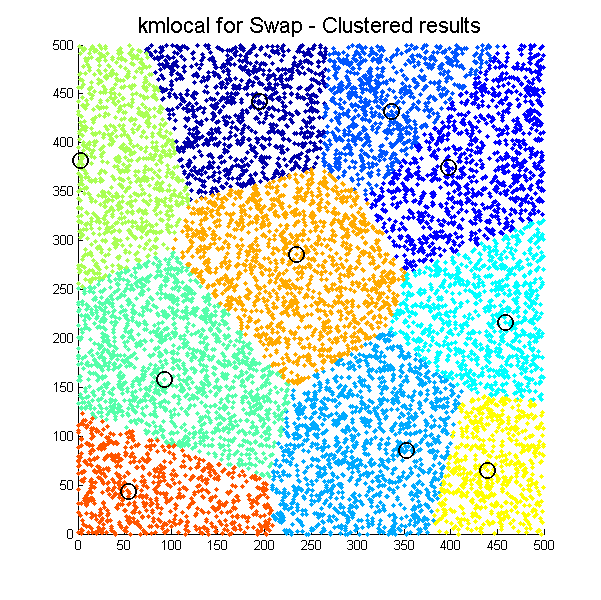
\includegraphics[scale=.5]{img/voronoi}
  \caption{K-vidurkių sugeneruoti klasteriai atitinka Voronoi diagramas\\
           Šaltinis: \url{https://summerofhpc.prace-ri.eu/quizz-clustered-data-using-k-means/}}
\label{img:voronoi}
\end{figure}

\subsubsubsection*{K-vidurkio algoritmo alternatyvos}

Dėl palygint paprasto veikimo principo ir populiarumo k-vidurkių
algoritmas susilaukė daug modifikuotų versijų. Keletas jų:

\begin{itemize}

\item
  \textit{K-Medians} – naudoja medianas vietoj vidurkių \cite{jain1988algorithms}. Šis metodas
  mažiau jautrus taškams atsiskyrėliams, bet yra lėtesnis.
\item
  \textit{Fuzzy C-means} – negriežta k-vidurkių versija \cite{dunn1973fuzzy}.
\item
  \textit{Bisecting k-means} – hierarchinė k-vidurkių versijak-means \cite{steinbach2000comparison} .
\end{itemize}






\subsubsection{Lūkesčių-maksimizavimo}

\ltang{Lūkesčių-maksimizavimo}{expectation–maximization},
(toliau EM) priklauso
\ltang{pasiskirstymo modelių}{distribution models}   grupei
ir dar yra vadinamas tikimybiniu klasterizavimo algoritmu.
Šis metodas
remiasi statistiniais pasiskirstymais,
todėl tinka dirbtiniams duomenų rinkiniams.
EM yra vienas garsiausių šios grupės algoritmų \cite{wu2008top} ir naudoja \ltang{Gauso mišinių modelį}{Gaussian mixture}. EM atveju duomenų
rinkinys yra modeliuojamas su nustatytu \ltang{Gauso pasiskirstymų}{Gauss distribution}  
skaičiumi, kuris yra atsitiktinai inicijuojamas, o jo parametrai yra
iteratyviai optimizuoti, kad geriau atitiktų duomenų rinkinį.

Šis metodas yra laikomas bendresniu k-vidurkių metodo variantu, todėl
turi daug panašumų: abu metodai randa lokalų maksimumą, todėl gali
prireikti paleisti kelis kartus su skirtingai inicijuotais parametrais.
Taip pat EM turi du skirtingus parametrus $k$ ir klasterių pradines
padėtis. EM sugeneruoti klasteriai yra negriežti ir kiekvienas taškas su
atitinkama tikimybe gali priklausyti visiems klasteriams. Jei norime
paversti griežtu klasteriu, tereikia kiekvieną tašką priskirti
klasteriui, kuriam jis priklauso, su didžiausia tikimybe.

Veikimo principas:

\begin{enumerate}

\item
  Parenkame $k$ Gauso pasiskirstymų pradines reikšmes.
\item
  Suskaičiuojame tikimybę, su kuria objektai priklauso kiekvienam iš
  pasiskirstymų (\ltang{Lūkesčių}{expectation} žingsnis).\label{em2step}
\item
  Pagal tikimybes pakoreguojame pasiskirstymus (\ltang{Maksimizavimo}{maximization} žingsnis).\label{em3step}
\item
  Kartojame \ref{em2step} ir \ref{em3step} žingsnius kol konverguoja (klasteriai nesikeičia tarp
  žingsnių).
\end{enumerate}

\begin{figure}[H]
	\centering
	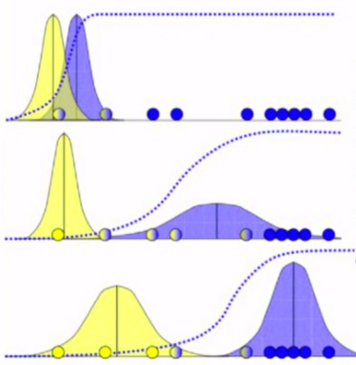
\includegraphics[scale=.5]{img/EM1d}
	\caption{EM pavizdys su vienmačiais duomenimis.\\
			     Šaltinis: \url{https://www.youtube.com/watch?v=iQoXFmbXRJA}}
\end{figure}


\subsubsubsection*{Parametrų parinkimas}

Naudojant EM iškyla ta pati problema kaip su k-vidurkių metodu – turime
iš anksto parinkti $k$, pradines klasterių padėtis ir parametrus.
Sprendimai iš principo yra labai panašūs į k-vidurkių, tik yra
sudėtingesni, nes EM klasteriai yra Gauso pasiskirstymai, kurie turi
daugiau parametrų nei centroidai.

\subsubsubsection*{Lūkesčių-maksimizavimo algoritmo savybės:}

\begin{itemize}

\item
  Sugeneruoja negriežtus, plokščius klasterius.
\item
  Teoretiškai konvergavimas gali užtrukti amžinybę, todėl reikia
  nurodyti nuo kokio minimalaus pasikeitimo nustoti ieškoti geresnio
  varianto.
\item
  Negarantuoja, kad konverguos globaliam maksimume.
\item
  Lengvai galime paversti į griežtus klasterius.
\item
  Galime turėti taškų, kurie pagal tikimybes tikėtina vienodai priklauso
  keliems klasteriams. Jei mūsų užduočiai tinka, galime šiuos taškus
  apibrėžti „tarpiniais“ ir nepriskirti jų nei vienam klasteriui.
\item
  Ne toks spartus kaip k-vidurkių metodas.
\item
  Rezultatai sunkiau interpretuojami nei taikant griežtus metodus.
\end{itemize}






\subsubsection{Hierarchinis}

\ltang{Hierarchiniai}{hierarchical}   klasterizavimo algoritmai yra
viena iš populiariausių dokumentų klasterizavimo algoritmų grupių, nes
nereikalauja iš anksto nurodyti klasterių kiekio ar \ltang{slenksčio}{threshold}.
Todėl jie grąžina bendrą visų klasterių tarpusavio
priklausomybių struktūrą ir tai leidžia nuspręsti koks klasterių
skaičius yra optimalus.\\
Hierarchiniai klasterizavimo algoritmai skirstomai į skaidymo ir
jungimo.

\subsubsubsection*{Skaidymo algoritmai}

\ltang{Skaidymo}{divisive} algoritmai – objektų
priskyrimą pradeda \ltang{iš viršaus į apačią}{top-down}.
Pradžioje visus objektus priskirdami vienam klasteriui, tada nuosekliai
dalindami į smulkesnius klasterius, kol galiausiai kiekvienas objektas
turi po atskirą klasterį.

\subsubsubsection*{Jungimo algoritmai}

\ltang{Jungimo}{agglomerative}   algoritmai – objektus priskiria
priešingai nei skaidymo – \ltang{iš apačios į viršų}{bottom-up}  .
Iš pradžių kiekvienas objektas priskiriamas atskiram klasteriui, tada
panašiausi klasteriai sujungiami, tai kartojama kol galiausiai turime
vieną klasterį.

\begin{figure}[H]
  \centering
  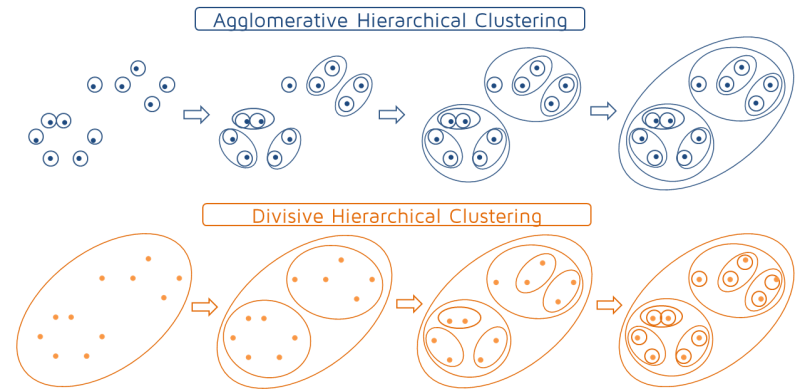
\includegraphics[scale=.5]{img/aggVSdiv}
  \caption{Grafinis pavizdys kuo skiresi jungimo nuo skaidymo algoritmai.\\
           Šaltinis: \url{https://quantdare.com/hierarchical-clustering/}}
\end{figure}

\subsubsubsection*{Atstumo matavimas / jungimo metodai}

Naudojant hierarchinio klasterizavimo metodą iškyla problema: kaip
išmatuoti atstumą tarp klasterių. Tam yra naudojami klasterių jungimo
metodai, kurie kai kuriuose šaltiniuose yra laikomi atskirais
klasterizavimo algoritmais. Keletą populiariausių jungimo metodų yra \cite{slaclc}:

\ltang{\textbf{Artimiausio kaimyno}}{nearest neighbor, single link}
 – atstumas tarp artimiausių
objektų atskiroje poroje klasterių Naudojant šį jungimo metodą, sudaromi
klasteriai įgauna ilgų objektų grandinių formą.

\ltang{\textbf{Tolimiausio kaimyno}}{furthest neighbor,
complete link} – atstumas tarp tolimiausių
objektų atskiroje poroje klasterių. Naudojant šį jungimo metodą,
sudaromi klasteriai įgauna sferinę formą.

\ltang{\textbf{Vidutinių atstumų}}{average link} –
vidutinis atstumas tarp visų įmanomų objektų
atskiroje poroje klasterių. Tai lėtai veikiantis, bet mažiau įtakojamas
taškų atsiskyrėlių, metodas.

\ltang{\textbf{Centroidų}}{centroids} – kaip ir k-vidurkių algoritme
 surandame visų klasterio objektų
centroidą ir tada pamatuojame atstumą iki kito klasterio centroido.

\textbf{Ward metodas}\footnote{Čia aprašyta \ltang{minimalaus pakitimo
  kriterijaus}{Minimum variance criterion} versija}

\begin{enumerate}
\item
  Apskaičiuojame kiekvieno klasterio centroidus ir $Cdis$ (taip kaip k-vidurkių metodas(\ref{km})).
\item
  Išmatuojame kiekvienos įmanomos klasterių poros naujus centroidus ir
  $Cdis$.
\item
  Jungiame tą porą klasterių, kurių nauja $Cdis$ reikšmė po
  sujungimo mažiausiai pasikeis.
\end{enumerate}

\begin{figure}[H]
  \centering
  \begin{subfigure}[b]{.3\textwidth}
    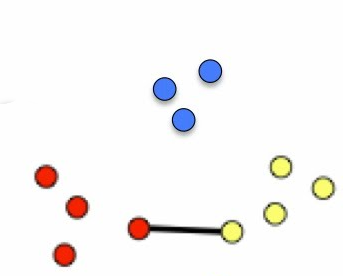
\includegraphics[scale=1]{img/single}
    \centering
    \caption{Artimiausio kaimyno}
  \end{subfigure}
  \begin{subfigure}[b]{.3\textwidth}
    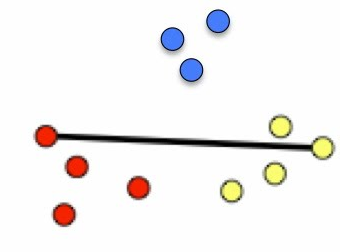
\includegraphics[scale=1]{img/complete}
    \centering
    \caption{Tolimiausio kaimyno}
  \end{subfigure}
  \begin{subfigure}[b]{.3\textwidth}
    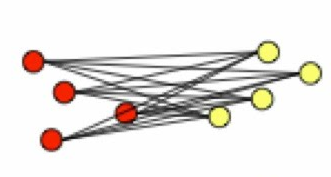
\includegraphics[scale=1]{img/average}
    \centering
    \caption{Vidutinių atstumų}
  \end{subfigure}
  \begin{subfigure}[b]{.3\textwidth}
    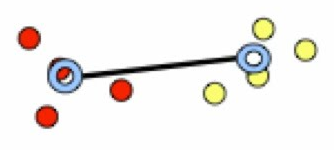
\includegraphics[scale=1]{img/centroid}
    \centering
    \caption{Centroidų}
  \end{subfigure}
  \begin{subfigure}[b]{.3\textwidth}
    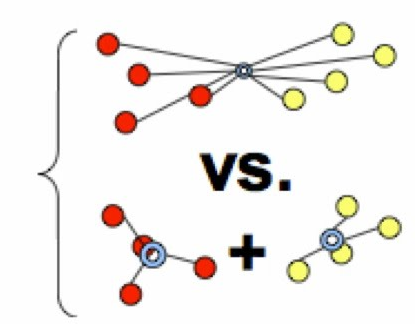
\includegraphics[scale=1]{img/ward}
    \centering
    \caption{Ward metodas}
  \end{subfigure}
  \caption{Atstumo matavimas / jungimo metodai.\\
  		     Šailtinis: \url{https://www.youtube.com/watch?v=vg1w5ZUF5lA}}
\end{figure}

\subsubsubsection*{Hierarchinių algoritmų savybės:}

\begin{itemize}
\item
  Skaidymo sudėtingumas – \BigO{2^n}, bet praktikoje naudojami
  heuristiniai metodai (kaip k-vidurkių) skaidymą pagreitina.\\
  Jungimo sudėtingumas – bendru atveju \BigO{n^3}, tačiau
  panaudojus \ltang{krūvos}{heap}   duomenų struktūrą, sudėtingumą
  galime sumažinti iki \BigO{n^2 log n}, jei naudojame artimiausio \cite{sibson1973slink}
  ar tolimiausio \cite{defays1977efficient} kaimyno atstumus, galima optimizuoti iki \BigO{n^2}.
\item
  Sugeneruoja griežtus, hierarchinius klasterius. 
\item
  Rezultatas – dendograma, kuri vaizduojama taip: x-ašyje išdėstyti
  dokumentai, y-ašies atstumas parodo klasterių skirtingumą: artimiausi
  klasteriai jungsis žemiausiai, o tolimiausi – pačiam viršuje. Norint
  gauti konkretų klasterių skaičių, „nupjauname“ dendrogramą
  pasirinktame lygyje.
\item
  Nereikia iš anksto nurodyti norimų klasterių kiekio ar 
 \ltang{slenksčio}{threshold}.
\item
  Reikia nurodyti papildomą atstumo matą.
\item
  Suteikia daugiau informacijos nei plokščiasis klasterizavimas.
\item
  Mažiau našus nei plokščiasis klasterizavimas.
\end{itemize}

\begin{figure}[H]
\centering
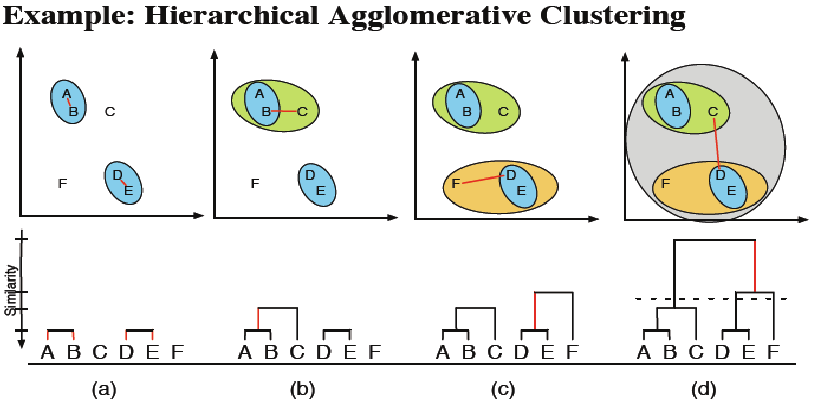
\includegraphics[scale=.5]{img/HierSteps}
\caption{Hierarchnio jungiamojo klasterizavimo pavizdys:\\
		 a) – Žingsnis rodo kaip sujungiami pavieniai obijektai į klasterius.\\
		 b) – Kaip prie klasterių prijungiami obijektai.\\
		 d) – Kaip galutinis rezultatas yra paverčiams į tris atskirus klasterius „atpjaunant“ dendogramą.\\
		 Šaltinis: \cite{janssen2012cluster}}
\end{figure}






\subsubsection{DBSCAN}

\ltang{DBSCAN}{density-based spatial clustering of applications with
noise} \cite{ester1996density} priklauso objektų \ltang{tankiu pagrįsto klasterizavimo}{density-based clustering}
metodų grupei. Taikant šį metodą
duomenys sugrupuojami į klasterius remiantis tuo, kad duomenys yra
pakankamai arti vieni kitų (tankūs). Tuo tarpu retai išsidėsčiusius
duomenis laikome \ltang{triukšmu}{noise}   ir nepriskiriame jokiam
klasteriui. DBSCAN tankį apibrėžia kaip taško aplinkoje (pagal parenkamą
spindulį) esančių taškų minimalų kiekį (parenkamas parametras).

DBSCAN reikalauja dvejų parametrų: $ε$ - maksimalus atstumas iki kaimyno
ir $MinPts$ – minimalus kaimynų kiekis.

DBSCAN taškai gali būti trijų rūšių: \ltang{\textbf{šerdiniai} taškai}{core points}
ir \ltang{\textbf{ribiniai} taškai}{border points}, kurie kartu sudaro klasterius,
 o \ltang{\textbf{atsiskyrėliai} taškai}{utliers} laikomi triukšmu.

Taisykės, pagal kurias taškai yra suskirstomi:

\begin{itemize}
\item
  Du taškai yra laikomi kaimynais, jeigu atstumas tarp jų yra mažesnis
  arba lygus $ε$.
\item
  Taškas yra laikomas \textbf{šerdiniu}, jeigu turi nors$minPts$
  kaimynų (įskaitant patį tašką).
\item
  Taškas yra laikomas \textbf{ribiniu}, jei turi mažiau nei
  $minPts$ kaimynų, bet vienas iš jų yra šerdinis taškas. 
\item
  Visi taškai nepasiekiami per bet kokį kitą tašką yra laikomi
  \textbf{atsiskyrėliais}.
\end{itemize}

Veikimo principas:

\begin{enumerate}
\item
  Atsitiktinai parenkame neaplankytą tašką $p$. Jei nebėra
  neaplankytų taškų stojame.\label{dbscan1steap}
\item
  Jeigu $p$ turi pakankamai kaimynų, jis tampa \textbf{šerdiniu}
  tašku ir sudaro naują klasterį:

  \begin{enumerate}
  \item
    Visi kaimyniniai taškai priskiriami klasteriui.
  \item
    Atliekame paiešką į gylį tarp neaplankytų klasterio taškų.\label{dbscan22step}

    \begin{enumerate}
    \item
      Jei aplankytas taškas turi pakankamai kaimynų, pažymime kaip
      \textbf{šerdinį} ir jo kaimynus pridedame prie klasterio. Grįžtame
      į \ref{dbscan22step} žingsnį.
    \item
      Jei aplankytas taškas neturi pakankamai kaimynų, pažymime kaip
      \textbf{ribinį}. Grįžtame į \ref{dbscan22step} žingsnį.
    \item
      Jei visi klasterio taškai aplankyti, grįžtame į \ref{dbscan1steap}-ą žingsnį.
    \end{enumerate}
  \end{enumerate}
\item
  Jei $p$ neturi pakankamai kaimynų jis tampa \textbf{atsiskyrėliu}
  tašku (jei vėliau paaiškės, kad vienas iš kaimyninių taškų yra
  šerdinis, $p$ taps \textbf{ribiniu} tašku). Grįžtame į \ref{dbscan1steap}-ą
  žingsnį.
\end{enumerate}

\begin{figure}[H]
\centering
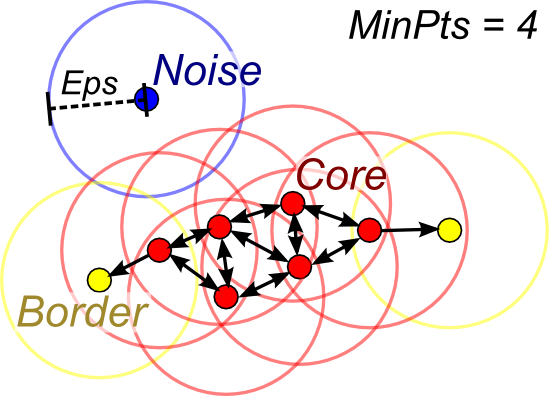
\includegraphics[scale=2.0]{img/DBSCANpts}
\caption{DBSCAN metodo taškų rūšys. Mėlynas – pašalinis, geltonas – pasienio, raudonas – centrini\\
		     Šaltinis: \url{https://stats.stackexchange.com/questions/194734/dbscan-what-is-a-core-point}}
\end{figure}

\subsubsubsection*{Parametrų parinkimas}
Idealioje situacijoje, jei dirbtume su fizinį pasaulį atitinkančiais
duomenimis, $ε$ reikštų fizinį atstumą tarp objektų, o MinPts laikytume
mažiausiu norimų klasterių dydžiu. Deja, tokie atvejai reti, todėl yra
kelios taisyklės kaip parinkti šiuos parametrus:

\begin{itemize}
\item
  $MinPts$ – minimalus kaimynų kiekis. $MinPts = 1$
  netinkama, nes tada kiekvienas atsiskyrėlis taškas turėtų atskirą
  klasterį. $MinPts = 2$ sugeneruotų tokį pat rezultatą kaip
  hierarchinio klaserizavimo metodas su sinlge link metrika ir
  dendrograma atkirpta ties $ε$ aukščiu. Taigi $MinPts$ reikšmė
  turėtų būti mažiausiai $3$. Kaip apytikslė taisyklė $MinPts = 2 \cdot dim$
  \cite{sander1998density}.
\item
  $ε$ - maksimalus atstumas iki kaimyno. $ε$ reikšmę galime pasirinkit
  naudojant \ltang{k-artimiausių kaimynų grafą}{k-nearest neighbor graph}
  (k-NNG). Taip pat alternatyviai DBSCAN versijai \ltang{OPTICS}{ordering
  points to identify the clustering structure} nereikia $ε$
  parametro, bet dėl to grąžinami klasteriai yra hierarchiniai.
\end{itemize}

\subsubsubsection*{DBSCAN algoritmo savybės:}
\begin{itemize}
\item
  Bendru atveju, sudėtingumas yra \BigO{n^2}. Jeigu duomenys patalpinti
  \ltang{erdviniame indekse}{spatial index}, sudėtingumas bus \BigO{n \log n}.
\item
  Sugeneruoja griežtus, plokščius klasterius.
\item
  Duomenims pakanka vienos iteracijos.
\item
  Nereikia iš anksto nurodyti klasterių skaičiaus.
\item
  Dirbant su tam tikrais duomenimis, parametrų parinkimas gali būti
  intuityvus, todėl atliekamas konkrečios srities eksperto.
\item
  Reikia iš anksto nustatyti 2 skirtingus jautrius parametrus, todėl net
  dėl mažo jų pasikeitimo, rezultatai gali labai skirtis (pvz.: \ref{sensitive} paveikslelis). Pavyzdžiui, per didelė $minPts$ reikšmė
  reikštų, kad maži klasteriai bus laikomi triukšmu. Esant per mažai $ε$
  reikšmei objektai bus sujungti į vieną klasterį.
\item
  Sudaryti klasteriai gali būti sudėtingų formų, vienas klasteris gali
  būti apsuptas kito klasterio (pvz.: \ref{shapes} paveikslelis).
\item
  Labai gerai susitvarko su taškais atsiskyrėliais.
\item
  Nesusitvarko su skirtingo tankio klaseriais.
\item
  Nėra visiškai deterministinis, nes priklausomai kokia eilės tvarka
  buvo parenkami ribiniai taškai, jie gali priklausyti skirtingiems
  klasteriams. Šią problemą išsprendžia
  DBSCAN* \cite{campello2015hierarchical}
  algoritmas, kuris ribinius taškus laiko triukšmu.
\end{itemize}

\begin{figure}[H]
  \centering
  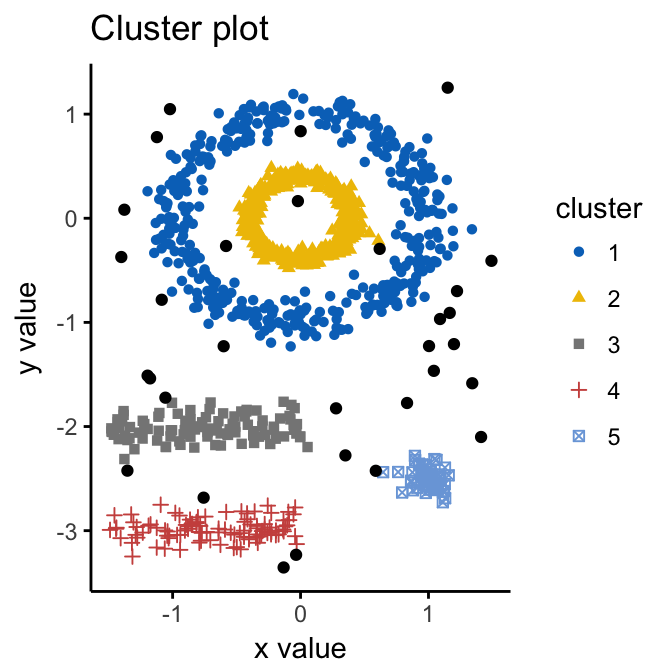
\includegraphics[scale=.3]{img/DBSCAN}
  \caption{DBSCAN sugeneruotų klasterių formų įvairovė.\\
           Šaltinis: \url{http://www.sthda.com/english/wiki/wiki.php?id_contents=7940}}
  \label{shapes}
  
\end{figure}

\begin{figure}[H]
  \centering
  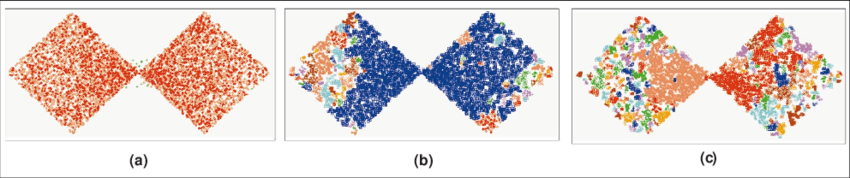
\includegraphics[scale=1]{img/DBSCANprob}
  \caption{Skirtingos ε reikšmės.\\
           Šaltinis: \cite{karypis1999chameleon}}
  \label{sensitive}
\end{figure}










\section{Kokybės vertinimas}

Visi klasterizavimo metodai turi bendrą silpnybę – jų paskirtis atrasti
duomenų struktūras, tačiau jie gali atrasti jas ir tais atvejais, kai
duomenyse nėra jokių struktūrų \cite{theodoridis2003feature}.
Todėl klasterizavimo kokybės \ltang{įvertinimas}{evaluation} yra
vienas svarbiausių klasterizavimo proceso etapų. Jo metu gauti
rezultatai parodo ar objektai (duomenys) buvo teisingai sugrupuoti į
klasterius be išankstinės informacjos apie grupes. Egzistuoja 4
kriterijai klasterizavimo rezultatų kokybei įvertinti \cite{feldman2007text}:

\begin{enumerate}
\item
  \ltang{\textbf{Vidiniai}}{internal} kriterijai kokybę vertina
  lygindami objektų vienoduose klasteriuose panašumą ir objektų skirtumą
  skirtinguose klasteriuose. Deja, šio tipo kriterijai nėra universalūs,
  skirtingiems klasterizavimo metodams reikia parinkti skirtingus
  vidinius kriterijus.
\item
  \ltang{\textbf{Išoriniai}}{external} kriterijai kokybę vertina
  lygindami gautus klasterius su jau iš anksto žinomomis duomenų
  klasėmis. Taigi, šiuo atveju vertiname neprižiūrimo mokymosi metodus
  su prižiūrimo mokymosi problemoms parengtais duomenimis. Nors labai
  tikėtina, kad neprižiūrimo mokymosi metodu sugeneruoti rezultatai bus
  blogesni, bet tai vis tiek labai vertingas vertinimo metodas. Tačiau
  svarbu atkreipti dėmesį, kad duomenis dažnai galima sugrupuoti keliais
  skirtingais būdais ir su duomenimis atėjusios \ltang{etiketės}{labels} 
  nebūtinai yra vienintelis galimas variantas. 
\item
  \ltang{\textbf{Rankiniai}}{manual} kriterijai, kai kokybė yra
  vertinama žmogaus. Praktikoje tokiu būdu visų sudarytų klasterių
  vertinimas užimtų labai daug laiko. Todėl dažniausiai vertintojui
  duodama pora objektų ir klausiama ar jie turėtų būti kartu, ar
  atskirai. Surinkę pakankamai rezultatų iš vertintojų, palyginame su
  rezultatais, gautais taikant klasterizavimo algoritmą. Taip pat šiuo
  atveju galima taikyti duomenų vizualizaciją, deja tai tampa ypač
  sudėtinga su didelės apimties duomenimis (tekstiniais dokumentais).
\item
  \ltang{\textbf{Netiesioginiai}}{indirect}
  kriterijai  įvertina  ar klasterizavimas yra vertingas žingsnis, didesnės
  problemos sprendimui   (pvz., klasterizavimas naudojamas vaizdų 
  atpažinimui  kaip tarpinis žingsnis matmenų kiekiui sumažinti ).
  Todėl galime  stebėti   didesnės problemos sprendimo  rezultatus
  su skirtingais klasterizavimo
  metodais  (ar jų parametrais) ir parinkti  tinkamiausią metodą.
\end{enumerate}






\sectionnonum{Išvados}

Kursiniame darbe buvo pasiektas užsibrėžtas tikslas – išnagrinėti ir
aprašyti klasterizavimo metodai, jų veikimas ir savybės. Taip pat
apžvelgtos panašumo funkcijos, tekstinių duomenų išgavimo ir jų
parengimo darbui su klasterizavimo algoritmais būdai bei kokybės
įvertinimo kriterijai.

Kursinio darbo metu surinkta ir išnagrinėta informacija apie dokumentų
klasterizavimą bus panaudota projektiniame darbe atliekant
eksperimentinį tyrimą. Taip pat projektiniame darbe planuoju išsamiau
aprašyti tekstų parengimą, klasterių vertinimą, bei įrankius reikalingus
šioms užduotims atlikti.






\printbibliography[heading=bibintoc] % Literatūros šaltiniai aprašomi
% bibliografija.bib faile. Šaltinių sąraše nurodoma panaudota literatūra,
% kitokie šaltiniai. Abėcėlės tvarka išdėstoma tik darbe panaudotų (cituotų,
% perfrazuotų ar bent paminėtų) mokslo leidinių, kitokių publikacijų
% bibliografiniai aprašai (šiuo punktu pasirūpina LaTeX). Aprašai pateikiami
% netransliteruoti.

\appendix  % Priedai
% Prieduose gali būti pateikiama pagalbinė, ypač darbo autoriaus savarankiškai
% parengta, medžiaga. Savarankiški priedai gali būti pateikiami kompiuterio
% diskelyje ar kompaktiniame diske. Priedai taip pat vadinami ir numeruojami.
% Tekstas su priedais siejamas nuorodomis (pvz.: \ref{img:mlp}).

\section{Klasterizavimo algoritmų vizualizacija}
\begin{figure}[!ht]
  \centering
  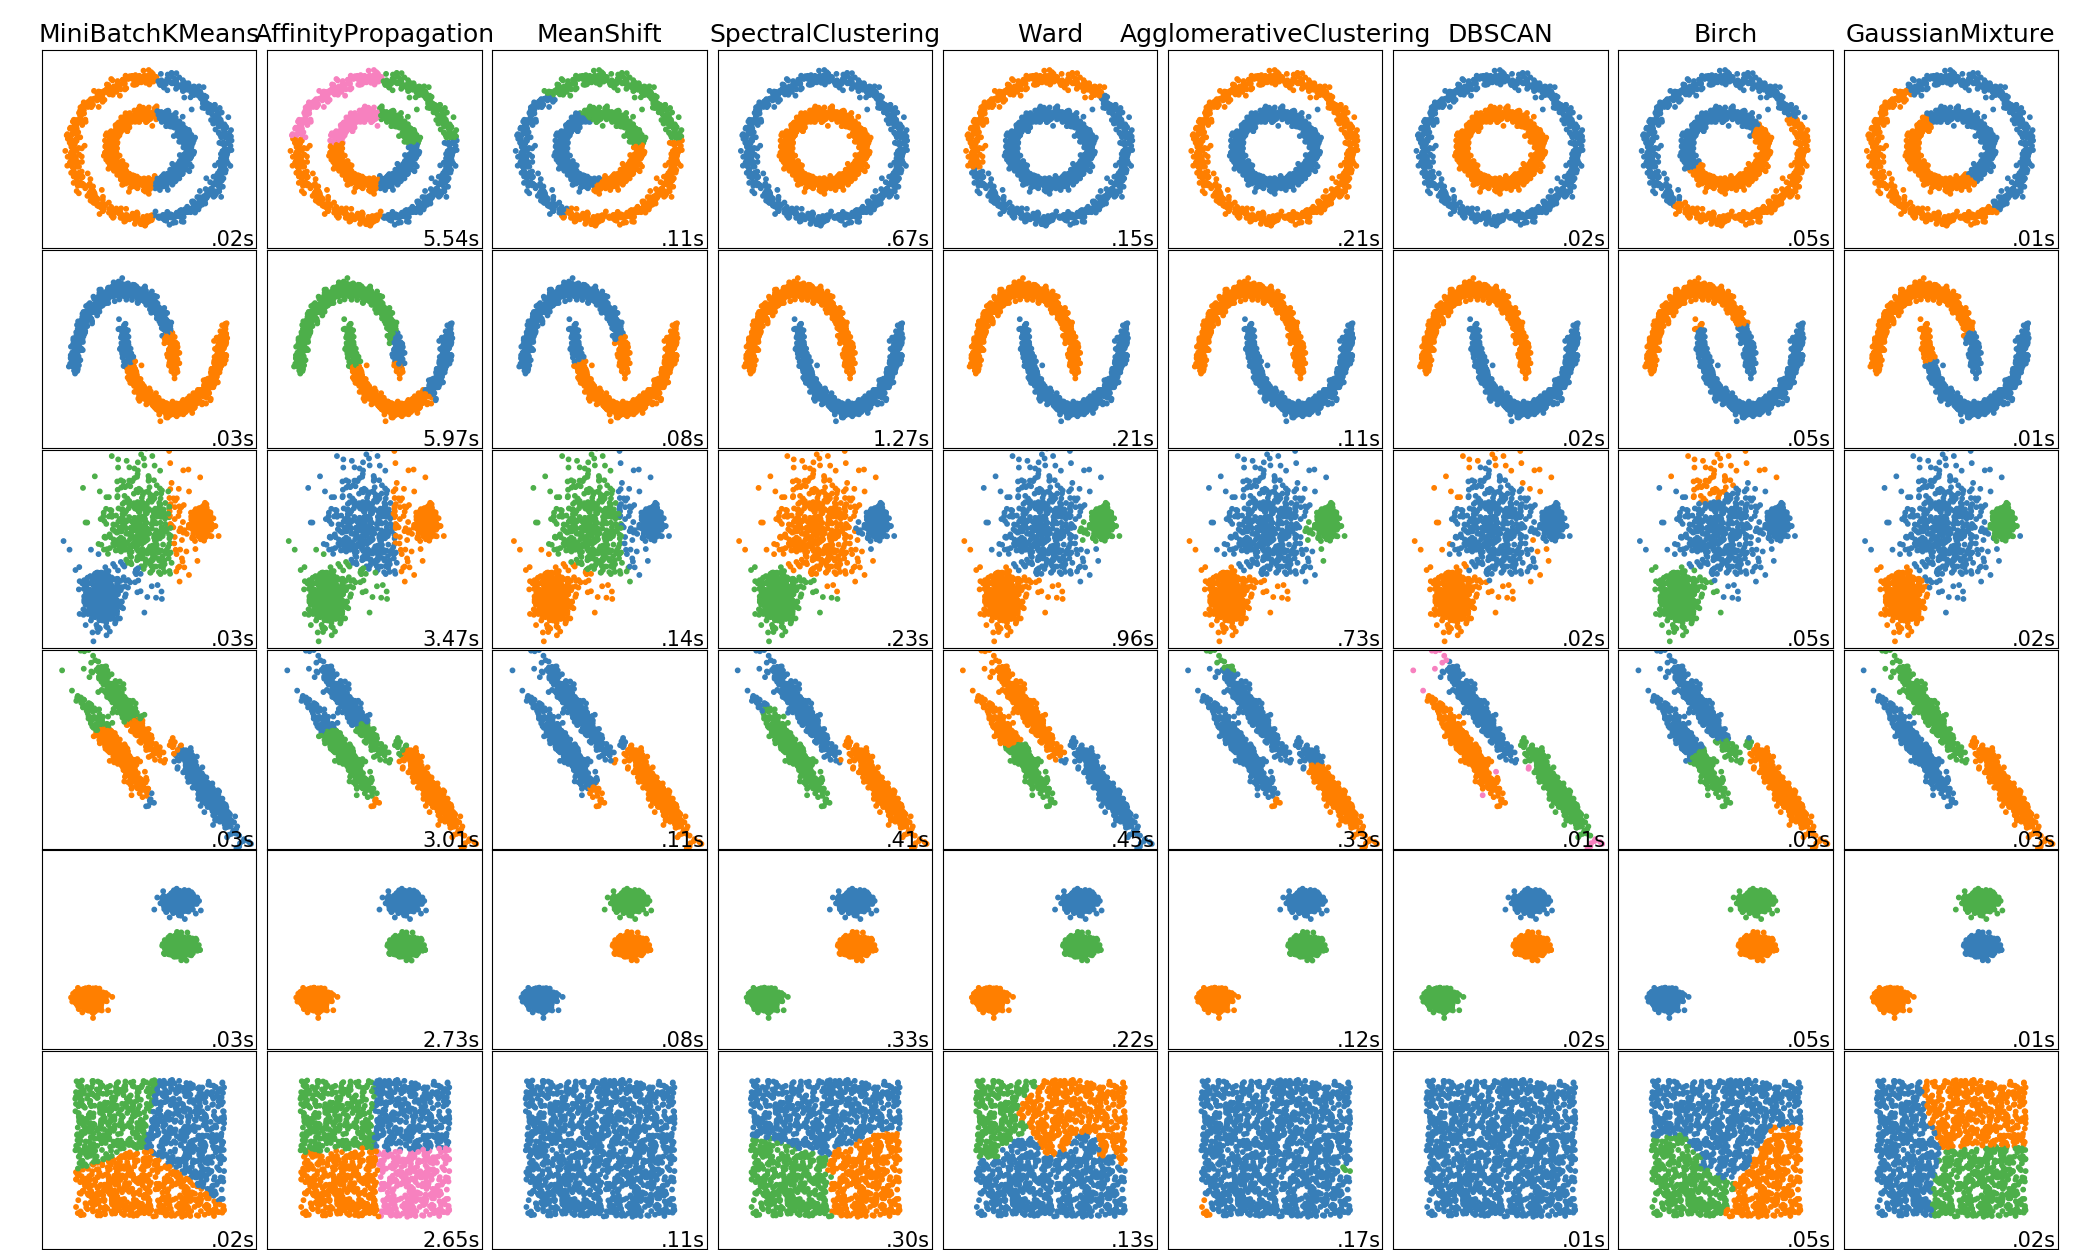
\includegraphics[scale=.3]{img/ClusterPlot}
  \caption{Klasterizavimo metodų palyginimas: MiniBatchKMeans – k-vidurkių;\\
   Ward, AgglomerativeClustering – jungiamasis hierarchinis; GaussianMixture – Lūkesčių-Maksimizavimo\\
   Šaltinis: \url{http://scikit-learn.org/stable/modules/clustering.html}}
  \label{clustAlg}
\end{figure}
%\clearpage

\end{document}
